\section{Saudi Arabian Grand prix}

\subsection{Circuit Analysis}

\textbf{Circuit Name:} Jeddah Corniche Circuit (Jeddah, Saudi Arabia) \\
\textbf{Length:} 6.174 km - \textbf{Laps:} 50 - \textbf{Total Distance:} 308.450 km

\begin{figure}[H]
    \centering
    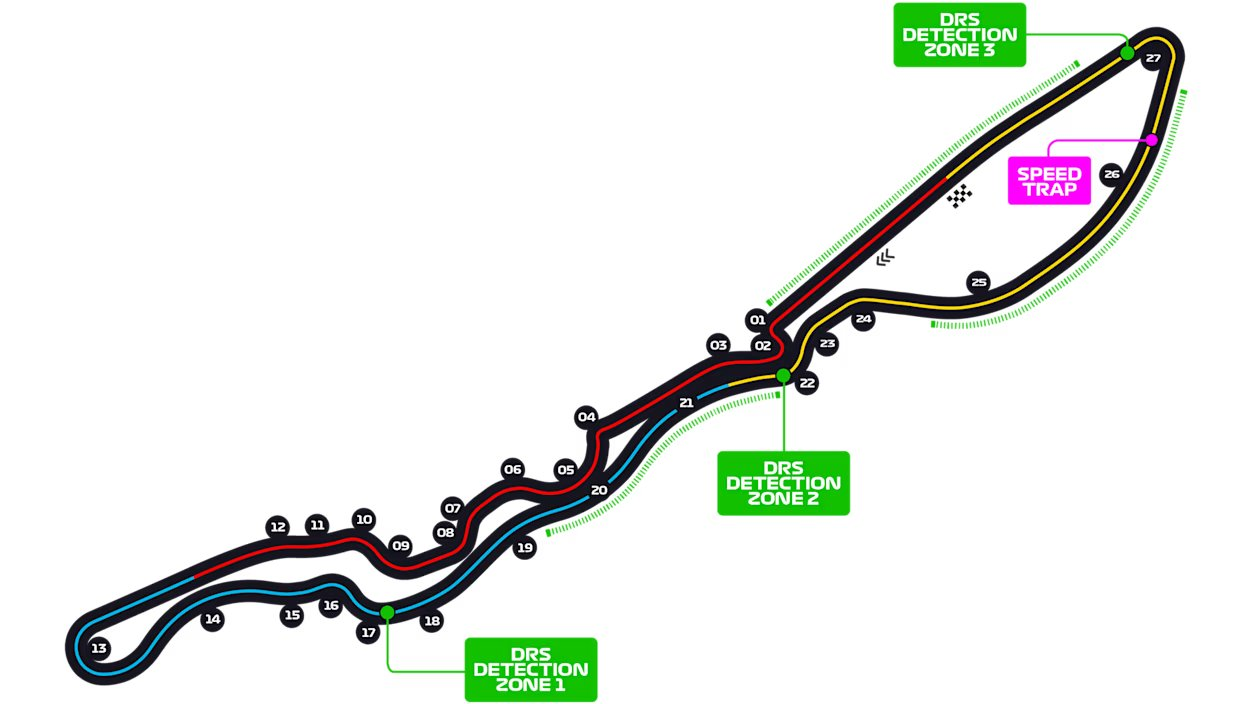
\includegraphics[width=0.75\linewidth]{images/2.Jeddah_Circuit.jpg}
\end{figure}

\begin{itemize}
    \item \textbf{Lap Record} : 1:27.511 (2021, Lewis Hamilton - Mercedes).
    
    \item \textbf{Number of Corners \& Key Features} : 27 turns (11 right, 16 left)  - High-speed kinks, extremely tight margins, walls very close to the track.\\
    Predominantly high-speed corners, including challenging sections like Turn 10 and Turn 22 with limited visibility.\\
    \textbf{Fastest corner (Turn 13)} can be taken at 322 km/h, with a 12° slope.
    
    \item \textbf{Braking Zones \& Traction} : Only 7 braking points per lap: 2 heavy, 2 medium, 3 light.\\
    \textbf{Most demanding zones:} Turns 1 (317→110 km/h), 22, and 27.
    
    \item \textbf{DRS \& Overtaking} : Three DRS zones: along main straight, near Turn 21, and before the final corner. \\
    Despite the DRS, only Turns 1 and 27 account for 89\% of overtakes in data.
    
    \item \textbf{Tyre Degradation \& Strategy} : Low tyre degradation allows one-stop strategies, especially with medium/hard compounds. \\
    High likelihood of Safety Car due to narrow corridors and close barriers.
    
    \item \textbf{Weather \& Environment} : Night race under powerful lighting; temperatures drop significantly at night, affecting tyre grip and brake cooling.\\
    Proximity to desert means wind and sand can affect grip unpredictably.
\end{itemize}

\textbf{Strategic Summary :}
The Jeddah track demands cars with engine power, straight-line speed, stability at high velocity, and precision through kink-heavy sectors. Overtaking is concentrated around heavily-braked zones, and teams must be ready for Safety Car-induced strategic shifts. One-stop strategies are usually viable, but environmental effects like sand dust and temperature swings cannot be ignored.


\subsection{Race Analysis}

\textbf{Date:} 9 March 2024 — 20:00 local time 

\begin{itemize}
    \item \textbf{Qualifying Summary} : \textbf{Pole Position:} Max Verstappen (Red Bull) – 1:27.472 (new track record). \\
    Grid: Leclerc 2nd, Pérez 3rd, Alonso 4th.\\
    Notable: Rookie Oliver Bearman (Ferrari, replacing Sainz – appendicitis) qualified P11.
    
    \item \textbf{Race Summary} : \textbf{Winner:} Max Verstappen (Red Bull). \\
    \textbf{Podium:} 1. Verstappen - 2. Pérez - 3. Leclerc.\\
    \textbf{Technical issues:} Gasly (gearbox - retired formation lap).\\
    \textbf{Notable incidents:} Stroll crashed at Turn 14 (Safety Car lap 7).\\
    Rookie Bearman finished P7 on debut, scoring 6 points for Ferrari.
    
    \item \textbf{Strategies} : 
    - Teams mostly opted for one-stop strategies, using medium tyres for the first stint.\\
    - Medium durability allowed extended stints. 
    - Some switched to softs late for speed.
    
    \item \textbf{Performance Trends} : \textbf{Red Bull} — Dominant again, securing a second 1–2 despite Pérez’s 5s penalty. Verstappen unchallenged (45 laps led). \\
    \textbf{Ferrari} — Leclerc maximised P3 + fastest lap. Rookie Bearman impressed with calm, consistent debut drive to P7. \\
    \textbf{McLaren} — Piastri P4, Norris P8, competitive but not podium-level. \\
    \textbf{Mercedes} — Russell P6, Hamilton P9, solid points but lack of pace in straights evident. \\
    \textbf{Aston Martin} — Alonso P5, Stroll retired after crash. \\
    \textbf{Haas} — Hülkenberg P10, first point of the year. 
    
    \item \textbf{Championship Impact} : \textbf{Drivers:} Verstappen 51 points, Pérez 36, Leclerc 28 (+1).\\
    \textbf{Constructors:} Red Bull 87, Ferrari 49, McLaren 28 (+1), Mercedes 26 (-1).    
\end{itemize}

\textbf{Key Takeaway :}
Verstappen extended his winning streak with complete control. Pérez salvaged P2 despite a penalty, while Leclerc and Ferrari optimised points. Bearman’s surprise debut and points finish provided the human highlight of the weekend.


\subsection{Link \& Takeaway}

\begin{itemize}
    \item High-speed layout perfectly matched Red Bull’s strengths in aero efficiency and straight-line speed. 
    \item One-stop strategy confirmed Jeddah’s low tyre wear, with little variation in pit calls. 
    \item Safety Car briefly reshuffled order but didn’t threaten Verstappen’s dominance. 
    \item Bearman’s debut became the story of the weekend, contrasting with Red Bull’s overwhelming control. 
    \item Overtaking limited to key braking zones, the safety car period (after Stroll's crash) didn’t significantly disrupt the top order.
\end{itemize}